\documentclass{beamer}

\usepackage{graphicx,hyperref,udesc,url}
\usepackage[utf8]{inputenc}
\usepackage[T1]{fontenc}
\usepackage{booktabs}
%\usepackage[portugues]{babel}
\usepackage{amssymb}
\usepackage[utf8]{inputenc}
\usepackage[brazil]{babel}
\usepackage{csquotes}
\usepackage{listings}
\usepackage{amsmath}
\usepackage{amsthm}
\usepackage{mathtools}
\usepackage{verbatim}
%\usepackage[table,xcdraw]{xcolor}
\usepackage{multirow}

\title[]{Otimizações para Motores de Jogos Através de Modelagem Orientada a Dados}

\author[Vinicius Bruch Zuchi]{
    Vinicius Bruch Zuchi\\\medskip
    {\small \url{vinicius.b.zuchi@gmail.com}\\}}

\institute[UDESC]{
    Departamento de Ci\^encia da Computa\c{c}\~ao \\
    Centro de Ci\^encias e Tecnol\'ogicas\\
Universidade do Estado de Santa Catarina}

\begin{document}

\begin{frame}
    \titlepage
\end{frame}

\begin{frame}
    \frametitle{Sum\'ario}
    \tableofcontents
\end{frame}

\section{Recapitulando}

\frame{\tableofcontents[currentsection]}

\begin{frame}[t]{Problema}
    \begin{itemize}
        \item Processadores possuem um alto poder computacional, porém o acesso à memória é relativamente lento
        \item Gargalo de desempenho na velocidade de acesso à memória
        \item Processador gasta muitos ciclos ociosos
    \end{itemize}
\end{frame}

\begin{frame}[t]{Motor de Jogos}
    \begin{itemize}
        \item Separação entre a parte técnica e criativa do jogo
        \item Conjunto de componentes que interagem entre si
        \item A interação cria os loops de jogo (inputs, atualização e renderização)
        \item Motivação: modularização, rápida prototipagem e desenvolvimento, e portabilidade
    \end{itemize}
\end{frame}

\begin{frame}[t]{Motor de Jogos}
    \begin{itemize}
        \item Jogos são notórios por possuirem um grande volume de dados
        \item Muitas entidades que necessitam de atualização e processamento
        \item Muitos dados sendo lidos da memória
        \item Se o agrupamento de dados não está coerente: poluição de cache
    \end{itemize}
\end{frame}

\begin{frame}[t]{Como Solucionar}
    \begin{itemize}
        \item Não há como aumentar a capacidade dos caches...
        \item O que resta aos desenvolvedores é organizar o código e estruturas de dados
              de tal forma a otimizar a leitura dos dados para uma linha de cache.
    \end{itemize}
\end{frame}

\section{Modelagem Orientada a Dados}

\frame{\tableofcontents[currentsection]}

\begin{frame}[t]{Origem e Popularização}
    \begin{itemize}
        \item Introduzido por John A. Sharp em 1980
            \begin{itemize}
                \item Seu objetivo era aprimorar o tempo de processamento e eficiência da memória
                \item Organização dos dados para permitir uma leitura sequencial destes
                \item Separação de dados quentes e frios
            \end{itemize}
        \item Popularizado como \textit{Data Oriented Design} por Mike Acton em 2009
        \item Surgimento de motores de jogos utilizando os conceitos de DOD
    \end{itemize}
\end{frame}

\begin{frame}[t]{Principais Ideias}
\end{frame}

\begin{frame}[t]{Como Armazenar os Dados}
\end{frame}

\begin{frame}[t]{Branching e Prefetching}
\end{frame}

\section{O Trabalho Desenvolvido}

\frame{\tableofcontents[currentsection]}

\begin{frame}[t]{Motivação}
\end{frame}

\begin{frame}[t]{Aplicações Desenvolvidas}
\end{frame}

\begin{frame}[t]{Etapas de Conversão}
\end{frame}

\begin{frame}[t]{Diferenças Entre as Abordagens}
\end{frame}

\begin{frame}[t]{Método de Renderização}
\end{frame}

\begin{frame}[t]{Método de Atualização}
\end{frame}

\begin{frame}[t]{Detecção de Colisões}
\end{frame}

\section{Análises e Resultados}

\frame{\tableofcontents[currentsection]}

\begin{frame}[t]{Cenários Desenvolvidos}
\end{frame}

\begin{frame}[t]{Problema A: Médias}
\end{frame}

\begin{frame}[t]{Problema A: Draw}
\end{frame}

\begin{frame}[t]{Problema A: Update}
\end{frame}

\begin{frame}[t]{Problema A: Collision}
\end{frame}

\begin{frame}[t]{Problema B: Médias}
\end{frame}

\begin{frame}[t]{Problema B: Draw}
\end{frame}

\begin{frame}[t]{Problema B: Update}
\end{frame}

\begin{frame}[t]{Problema B: Collision}
\end{frame}

\section{Conclusão}

\frame{\tableofcontents[currentsection]}

\begin{frame}[t]{Diferença de MOO e MOD}
    \begin{figure}
    \centering
        \begin{minipage}[b]{0.35\textwidth}
            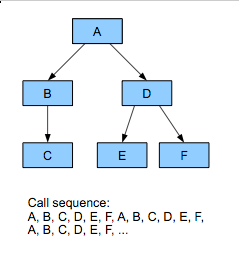
\includegraphics[width=\textwidth]{figuras/objectreadingorder}
        \end{minipage}
        \begin{minipage}[b]{0.35\textwidth}
            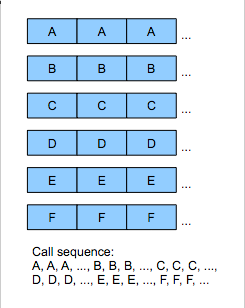
\includegraphics[width=\textwidth]{figuras/dodreadingorder}
        \end{minipage}
        %\par\medskip
        %Disponível em: <http://gamesfromwithin.com/data-oriented-design>. Acesso em: 27/05/2017.
        %\label{oodvsdod}
    \end{figure}
\end{frame}

\begin{frame}{Fim}
    \centering
    \LARGE{That's All Folks!}
\end{frame}

\end{document}
